

%\maketitle


\section{Abstract}
In the last decade the amount of data being created has increased incredibly.  
,,Industrial Revolution of Data''\cite{aobd} is driven by explosion of cheap and numerous data gathering mobile devices, servers continuously 
logging messages about what they are doing, and by the emerging IoT. And above all the ultimate source of information, the Internet is almost incomprehensible enormous.
This revolution profoundly influences the rules of the information business, the traditional informational systems, 
like relational databases are pushed to their limits and in an increasing number of cases systems collapses under the pressure of Big Data.\cite{marz}
As Big Data infrastructures became widely used, users of ,,Big Data'' then started expecting fresh, low latency results, above processing large volumes of data. In response to this demands the new breed of distributed applications has emerged, the  class of \textit{Distributed  Stream  Processing Systems}(DSPSs).

As distributed systems in general DSPSs must comply with a number of base requirements, they have to ensure high availability, robustness against failures, and have to provide correct results.  
This paper is dedicated to examining how DSPSs can achieve resilience against failures at iterative computations, and how it influences efficiency of the computations in machine learning problems.
First part of this paper is meant to describe the context of iterative fault tolerance, from the emerge of \textit{Big Data}(Section ~\ref{bigdata}), through architectural principles of distributed stream based applications (Section ~\ref{streaming}), to an overview of recovery techniques in already implemented systems (Section ~\ref{ft}). 

The experiments described in the second part of the paper are executed using \textit{Apache Flink}(Section ~\ref{flink}) on the implementation of \textit{linear regression} (Section ~\ref{linearregression}). Some  Machine Learning problems as well as linear regression, have the characteristic that they are able to reach convergence from only a subset of input data.  Another experiment aims to discover the impact of recovery using exactly once processing guarantees.   
     
\section{Big Data}\label{bigdata}
The appellation ,,Big Data'' is today one of the most hyped buzzword in information technology. The phenomenon behind the name can be described either 
as data sets whose sizes  exceed the capabilities of traditional management techniques, or data moving too fast to keep up with it in a scaleable and 
conststent manner. In 2001 Doug Laney defined challanges posed by databoom as being three dimensional\cite{3v}. The three main aspect of Big Data in Laney's summary was:
\begin{description}

\item[Volume:]
 the most obvious aspect is the increased volume of data, caused by transaction volumes and other traditional data types as well as by new data types. 
Though too much data itself involves a massive storage and analyzes issue, but as \textit{Gartner's} people warned\cite{3v},  enterprises should not exclusively focus on volume problems excluding many other aspect. Ignoring other dimensions of Big Data problem at restructuring  informational infrastructures may lead to massive reinvestment in couple of years. 
\item[Variety:] \textit{Revolution of data} added a number of new information sources to traditional database architectures, as social media contents , emails,  metering data, 
computer logs, images and so on. Informational systems need to be able to work with these partially or differently structured data sources. 
\item[Velocity:] Velocity means how fast data is produced and how fast it needs to processed. Problems like how to create structured data and
 how to access and deliver it also need to be addressed.
\end{description}
To this \textit{3V} description of big data two new dimension were added later, like \textit{Variability}, means that data often get to an inconsistent state what hampering precise processing, and \textit{Veracity}, which indicates that quality of data can vary greatly. 

Big Data is created anyway. Handling new magnitude and nature of datasets would involve an almost impracticable complexity with traditional approaches ,
 therefore rethink data systems from ground up became necessary. The desired properites of a Big Data informational system\cite{marz} are
 \begin{description}
\item[Robustness and fault tolerance:] System needs to behave correctly in an environment where the failure of components is rather rule than exception.
\item[Low latency reads and updates:] Usually the applications requires reads with very low latency, while update latency needed depends on nature of task.
\item[Scalability:] Maintain performance in face of increasing data is crucial property of Big Data systems. 
\item[Generalization:] Big Data infrastructures need to be able to support as wide range of applications as possible.
\item[Extensibility:] Adding a new feature to a working system must be as easy and cheap as possible.
\item[Minimal maintenance:] To minimize costs of keeping running the application smoothly users possibly has to build on components with little 
complextity provided by the infrastructure.
 \end{description}
Tuckle the challenges posed by data revolution, and convert large, fast moving, diversely collected and structured pile of data into \textit{Value} brought to life an entirely new a new breed of technologies, complying more or less with the introduced requirements. 
As solution for Big Data problems evolved distributed file systems, NoSQL databases, and distributed data processing technologies. 

Many of these new techniques were developed by Google like the distributed Google File System\cite{gfs} or MapReduce\cite{mapreduce} computational framework atop of it. 
Another pioneer was Amazon with it's innovative distributed key-value store \textit{Dynamo}. The open source community followed them in a couple of years with 
developing of Hadoop, HBase, MongoDB, Cassandra and many other systems.

For any Bid Data related distributed system the ability to scaling out is an essential need. That means that that system has to be able to provide nearly the same performance 
only by added new machines to the cluster. On storage layer the database is splitted into shards stored in different machines. As the systems grows the probability of a component will fail increases as well, 
therefore distributed storage systems uses replicas of the shard also distributed in the cluster.

Moving our databases into a distributed environment inevitable leads to releasing \textit{ACID properties}.  As \textit{Eric Brewer} described, 
there is a fundamental trade-off between consistency, where reads are guaranteed to see all writes done before, and availability where every query 
can be answered instead of failing (\textit{CAP theorem}). 
 
Systems can use consistency over availability, but then they face some inconvenient issues. In this case the main question is how to handle writes.  
The system has to ensure that whatever datanode answers the query the result must be always the same. This can be achieved through caching write requests until all replicas can be updated. But apart from the menace that all writes will be lost when the buffering machine falls out, this brings up another type of inconsistency, 
namely that client thinks that the database is updated with its write, while new data is still in buffer.  
The other option is keeping in focus availability. In this case multiple read at same time can give different results depending on which data node answered the query. 
It is on the developer to resolve inconsistency but maintain eventual consistency in such a system easily can mean too heavy of a burden for developers.


Distributed computational systems built atop distributed data storage two main approach for data processing, \textit{batch processing} and \textit{stream processing}. Batch processing provides a different 
manner of executes queries comparing to traditional SQL approach. When one works with relational databases usually uses an incremental computation techique,
 namely when new data comes in, the response to the query will be computed by updating the former result with the new entry. Alternatively it is possible 
 to use recomputational algorithms, which throws away previous results and recomputes the answer each time by reading over the entire dataset. 
 The leading computation model in data intensive recomputational tasks is MapReduce originally developed by Google to support processing data stored in GFS.
 A MapReduce program consists of three main phase, the input data is transformed into key - value pairs locally using Map function, than in the Shuffle phase results of Map are redistributed between worker nodes based on keys. Reduce functions then 
process data per key in parallel. Batch processing meet almost all the requirements an informational system has to comply with, and because 
 of its distributed nature also can provide high availability. Nevertheless these systems has the clear drawbacks, the always big latency, and due to this always 
 presenting \textit{latency} in case of continuous writes even \textit{eventual consistency} is too hard to reach.
  
\textit{Nathan Marz} in 2011 in his blog post\cite{beatCAP} proposed a way to bypass the CAP theorem, and to get rid of drawbacks recomputational MapReduce based informational systems. %%lehetne képlet NM cikkből
 The system described by Marz as \textit{Lambda architecture}(Figure ~\ref{fig:lambda}) suggests, is composed by three layers, \textit{Batch layer}, \textit{serving layer} and \textit{speed layer}. Batch layer is is the level of distributed datasets composed from immutable 
atomic units, and serving layer is a set of views continuously recomputed from the underlying datastrorage. To bridge latency rooted in total computation Marz introduces speed layer processing new data written after last data consumed by serving layer.
This last speed layer uses \textit{streaming}, another concept of data intensive technologies which aims processing data instantly.

\begin{figure}[!ht]
  \centering    
      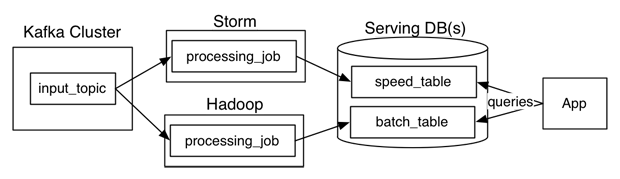
\includegraphics[width=0.9\textwidth]{figures/lambda-architecture.png}
  \caption{Lambda architecture \cite{beatCAP}}
  \label{fig:lambda}
\end{figure}
%% ábra http://radar.oreilly.com/2014/07/questioning-the-lambda-architecture.html
 
\section{Streaming concepts } \label{streaming}

Streaming --if we define it according to type of data-- is a processing technique, that is designed with infinite data sets in mind.\cite{101}. The colloquial use of term Streaming covers two different concepts as well as this definition, micro-batch processing and true streaming.
The key distinction data between data they process is about finiteness, or rather how we regard it.
\begin{description}
\item[Unbounded data:] a continuously growing essentially infinite data set, often referred a streaming data. Unbounded data processing is a continuous data processing.
\item[Bounded data:]finite dataset, the input of batch processing.
\end{description}
Nowadays data scientists like \textit{Jay Kreps} and \textit{Tyler Akidau} started questioning necessity of lambda architecture, stating that well designed streaming engines can do work of batch processing as well.  Jay Kreps came up with so-called \textit {Kappa- architecture}(Figure  ~\ref{fig:kappa}), where the batch phase is carried out by streaming engines too, using the same processing pipeline.
\begin{figure}[!ht]
  \centering    
      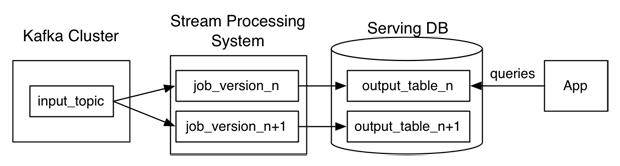
\includegraphics[width=0.9\textwidth]{figures/kappa-architecture.png}
  \caption{Kappa architecture \cite{beatCAP}}
  \label{fig:kappa}
\end{figure}
%% ábra http://radar.oreilly.com/2014/07/questioning-the-lambda-architecture.html
Nevertheless Akidau made a step further arguing in his blog post that well-designed streaming systems actually provide a strict superset of batch functionality, and saying there should be no need for batch systems as they exist today.
Replacing batch processing with streaming on entire filed of big data processing needs streaming engines to have a couple of substantial virtues. 

\subsection{Time }
One important characteristic related to this is about reasoning about time, which is an additional capability comparing to Batch systems, and is about how to bridge possible skews between event time and processing time. Some use cases just does not care about event time but many do. Based on their relation with time streaming tasks can be divided in three classes.

\paragraph{Time agnostic approach} means that time of events is essentially irrelevant. This processing manner is supported by any streaming engine. Such  \textit{data driven operations} are for example filtering, where we merely discard irrelevant data, or hash/inner join which is only interested in group data elements coming from different source. 
\paragraph{Approximation algorithms} have already some time aspect, but usually this is inside the logic of algorithms, the stream processing is still time agnostic.Finding approximate top-N problems belong here as an example (Top 5 videos watched in last 2 hours, or Top 10 news stories browsed in last 15 minutes ), where we want the answer in real time as soon as data arrived, and we are not really intereste in exact values.\cite{trend}
Approximation can be used for dynamic pattern identification algorithms like streaming k-means \cite{kmean}.
\paragraph{Time windows} The last concept concerned with time is windowing where the aim is to process data based on time it has been created or discovered. Windowing means processing data chopped up along temporal boundaries. Windows has three basic type \textit{fixed windows}, \textit{sliding windows} and \textit{sessions}. As its name suggest \textit{fixed windows} slice up time into fixed disjoint slices. 
\textit{Sliding windows} are a kind of generalization of fixed windows, they are defined by fixed length of window and a time gap between subsequent windows. When period between two windows equals the length of windows sliding windows are identical with fixed windows, while if the gap are longer than window's time span it results in a kind of sampling.
Using \textit{sessions} is an example for application of dynamic windowing most often used for examining users' behavior over time. Sessions are sequences of events which are terminated either by a final event or by an inactive period of a predefined length.

\paragraph{Watermarks}If the system works with times in which a particular event happened a common problem is how to deal with late data. In an ideal case events would be processed at time they occurred, but in reality they appear for the system with some smaller or bigger latency. Streaming systems handle this problem with the concept of watermarks. Watermarks are for measuring the progress and completeness of processing data originated in a given time period. They mark the time when we regard a given time span as all event occurred in it is arrived and processed. If we have a good knowledge of input it is possible to use perfect watermarks marking that after the watermark there is not relevant data anymore. Otherwise we can use heuristic watermarks use available information on the input and provides an estimation based on that.
Heuristics can be remarkably powerful but in case of use this concept the danger always given to meet late data. 

\paragraph{Triggers} To address the issue of late data we can use triggers. This mechanism allows us to define when the system should emit the output of a given window as well as update the fromerly issued output when late data arrives. \cite{102}
    
\subsection{State}
The other crucial thing is correctness, or how these systems do achieve textit{exactly once semantics}, which is the key advantage of batch computing over first streaming engines. A key structure which is necessary to do accurate computations is \textit{state}.
Streaming data processing can be divided into two basic group according to what supposed to happen to them some function executed on them. 
\paragraph{Stateless processing} In case of transformations are interested in only one record at time without needing to remember anything else, like filtering or MapReduce's map like functions can be stateless operations. \cite{localstate}
\paragraph{Stateful processing}
If the function needs to be executed uses some aggregation of data rows or joining together data from multiple streams then maintaining some state of the operator becomes necessary. 
State is store-able in two different way. One possibility of processing streams is to store states in a common remote database. The job takes input records from its input,and for each input records remotely calls the database. 
When we use partitioned input stream, it gives the opportunity to co-partitionate processing and the distributed database, which moves data to be directly co-located with processing (local state).
use of Local state has a huge efficiency benefit, since response time of remote calls is almost incomparable with local memory or disk access, not mentioning emerging throughput issues.
Nevertheless moving data to jobs raises reliability problems, namely  how to deal with machine failures.\cite{localstate}
Some streaming models using finite windowing like relational stream model(ilpubs.stanford.edu:8090/549/1/2002-41.pdf) uses operators with small amount of state, and current state depends on only the last couple of tuples. The more recent streaming data flow graph models provide users a way to implement incremental processing of large datasets permitting them to use so-called \textit{black box operators}, which can maintain arbitrary state potentially depending on the entire history of the stream. \cite{pietzuch:intscaleoutandft}  


\subsection{Streaming architecture, querying }
\subsubsection{System model}
A distributed computing system consists processes physically separated in space, that do not share a common memory and communicate with each other asynchronously, through passing messages over some communication channels. Each process and communication channel of the system has its  own state. A state of a process depends on the entire history of messages it received and all the computations it has executed. State of a process is characterized by the messages sent along it less messages received by all the  target processes.
\cite{introsnapshot}
\paragraph{Streaming data model}
We refer to the sequence of messages sent along a channel as \textit{stream}. A \textit{stream} \begin{math}s\end{math} is an infinite series of tuples \begin{math}t\in s\end{math}. A \textit{tuple} \begin{math}t=(\tau,k,p)\end{math} in general case consists of a logical timestamp $\tau$, a key field \(k\) and the payload \(p\).

 Tuples in stream are ordered according to their timestamp $\tau\in\mathbb{N}^{+}$ assigned by a monolitically increasing logical clock. The timestamp is set at the moment of creation of the tuple in the stream. \textit{Key} fields in the tuples are not unique, they are used to disrtibute records among working nodes of the system.\cite{pietzuch:intscaleoutandft}

\paragraph{Operator model}
Tuples are processed by \textit{operators}(processes). An operator $o$ takes $n$ \textit{input streams} $I_o=\{s_1,\dots,s_n \}$, processes their tuples and produces one ore more \textit{output streams}, $O_o=\{o_1, \dots, o_m\}$. Elements of the $I_o[\overline{\tau}]$ vector denotes series of tuples from input streams created before  the corresponding timestamps, namely they have timestamps less than $\overline{\tau}$, where $\overline{\tau}=(\tau_1,\dots,\tau_n)$  are the timestamps of  $I_o=\{s_1,\dots,s_n \}$ input streams.				
An \textit{operator function} $f_o$ defines the processing work operator $o$ has to execute on tuples of input streams:
\begin{equation}
f_o : (I_o, \overline{\tau_o},\theta_o,\overline{\sigma_o})\to (O_o, \overline{\tau_o}',\theta_o',\overline{\sigma_o}'),
\end{equation}
where $\overline{\tau_o}$  are timestamps of the most recent processed tuples, $\Theta_o$ is the state of the operator (in case of stateful operators), and $\overline{\sigma_o}$ specifies the oldest tuple affected state $\Theta_o$.
The operator function at each invocation accepts a finite set of tuples from the input stream $I_o[\overline{\tau_o}]$, and processes the input tuples. After processing, the operator advances to new positions on input streams and updates the value of $\overline{\tau_o}$ as well as  $\overline{\sigma_o}$ if it has changed from some reason, and computes the new $\theta_o'$ state. Stateless operator's state can be considered as constant $\Theta_o=\emptyset$.
The state of operators depends only on tuples with timestamps $\overline{\sigma_o}_i  \leq \overline{\tau}_i \leq \overline{\tau_o}_i$ for each $s_i$ input stream. \cite{pietzuch:intscaleoutandft}
\paragraph{Queries in streaming}
In streaming systems a query is defined as a directed \textit{query graph} $ q= (\mathcal{O},\mathcal{S})$, where $\mathcal{O}$ denotes the set of operators and $\mathcal{S}$ is the set of streams. Operators are nodes of the graph, while $s \in \mathcal{S}$ stream is represented as a directed edge of the graph ($s=(o,o')$ where ${o,o'}\in \mathcal{O}$). 

An operator $u$ is called \textit{upstream} to operator $o$, when $\exists(u,o) \in \mathcal{S}$, and similarly $d$ is a downstream of $o$, when $\exists(o,d) \in \mathcal{S}$. The sum of upstreams and downstreams of operator $o$ is denoted by $up(o)$ and $down{o}$.

Queries has two special type of operators, \textit{sources} ($src$: $up(src)=\emptyset$ )and \textit{sinks} ($snk$: $down(snk)=\emptyset$) of the data streams.\cite{pietzuch:intscaleoutandft}
%%piezuch ábra fele
\paragraph{Query execution} 
In stream processing systems a query is deployed on a set of nodes. We can assume that a node runs on one operator. Though in fact it is usually not true, it doesn't change the base concept. According to it's query graph we can distinguish between the logical representation of the query and the physical realization.

In physical \textit{execution graph} $\overline{q}$ an $o$ operator can be deployed on a set of nodes to partition the workload depending on a given hash function. $o^1,\dots,o^{\pi}$ partitioned operators implements the semantics of $o$ and process $s^1,\dots,s^\pi$ partitioned streams derived from an original $s$ input stream. 

The execution graph of a query either can be constructed in a static way from logical execution plan at the building up phase of query deployment or can be maintained dynamically by a query manager at runtime, Though this clearly more flexible and efficient approach requires a bit more sophisticated state handling comparing to static operator deployment.\cite{pietzuch:intscaleoutandft}
\begin{figure}[!ht]
  \centering    
      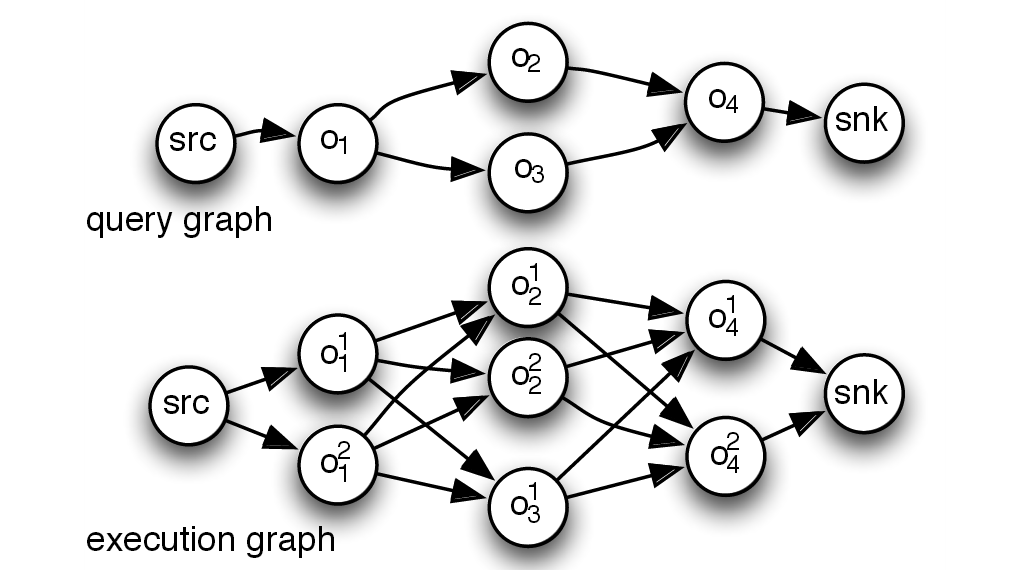
\includegraphics[width=0.5\textwidth]{figures/query_exec_graph.png}
  \caption{Query garph and execution graph \cite{pietzuch:intscaleoutandft}}
  \label{fig:gradient_descent_error_surface}
\end{figure} 
%%piezuch ábra fele
\subsubsection{State management}
State management in stream processing is often considered an implementation detail and used only for specific purposes, such as persistence or overload handling. Another approach is to make state of operators externally visible to the stream processing system. This second way of use of operator state yields several advantages regarding to scaling out as well as  to recovery after failures.
State of a query is composed by state of each operator. \textit{Operator state} can be divided into \textit{processing state}, \textit{buffer state} and \textit{routing state}. Each of these state has it's own important rule in maintaining or increasing efficiency of processing work.
\paragraph{Intra-query parallelism, scaling out}
Predicting the workload, a stream processing system needs to cope with, is not always a simple task, and at runtime of the systems increasing the throughput of computationally expensive queries could become necessary to avoid emerge of bottlenecks. To scale out dynamically the system needs to be able to identify the operator limiting the processing throughput of the query, which can be challenging in case of using more complex execution graphs. After finding of slowing down nodes a new issue comes up, namely how to reconfigure the execution graph without affecting the correctness of the result. If we use stateful operators the state of the logical operator needs to be partitioned as well.
\paragraph{Processing state}
Stateful operators compute their output streams from the tuples of input streams and from the sum of past tuples.
The term of \textit{processing state} covers the summary of history of these formerly processed tuples  typically maintained by the operator. $\Theta_o$ current processing state of operator $o$ is computed from all past tuples with time $\overline{\sigma_o}_i \leq \overline{\tau}_i \leq \overline{\tau_o}_i : s_i \in I_o $. 

Based on the data model introduced above the processing state of an operator $o$ can be described as a set of key-value pairs, $\Theta_o=\{ (k_1,v_1),\dots\}$, where each unique $k$ key refers to corresponding tuple keys, while $v$ denotes a set of  processing states required for processing tuples with $k$ key. Processing state is associated with a list of $\overline{\tau_o}$ timestamps returned by subsequent executions of $f_o$ operator function.
Naturally the operator doesn't have to maintain operator state using the described structures, and it can use more efficient manner of store this data, but the developer of the operator should implement a function which returns with the $(\Theta_o,\overline{\tau_o})$ vector pair for $o$ operator. 

Exposing processing state to streaming system, speeds up recovery after failures since makes unnecessary reprocessing  all tuples int the timestamp-range $\overline{\sigma_o}_i \leq \overline{\tau}_i \leq \overline{\tau_o}_i$. Moreover seeing state from the point of view of stream processing system provides the possibility to redistribute state across a set of new partitioned operator when the system scales out.
\paragraph{Buffer state}
A stream processing system typically places output buffers between operators, to collect tuples before sending them to the downstream operators. These buffers compensate the transient fluctuation of stream rates and network capacity. These buffers stores tuples not have been yet processed by downstream operators, therefore in case of  failure they must be reprocessed (????)/ should be reprocessed without externalized and backed-up state.
After dynamic scale out content of the buffer must be sent to the correct partitioned downstream operator.  If $d \in downstream(o)$ is a partitioned downstream operator of $o$, and  $\beta_o(d^i)$ refers to output tuples should be dispatched to  partitioned $d^i$ downstream operators, the structure of the state of output buffer $o$ can be the following:
\begin{equation}
\beta_o=\{\beta_o(d^1),\beta_o(d^2),\dots\}=\{(d^1,\{t_{1_1},t_{1_2},\dots\}),(d^2,\{t_{2_1},t_{2_2},\dots\}),\dots\}, 
\end{equation}
where $\beta_o(d^i) = \{t_{i_1},t_{i_2},\dots\}$ are  tuples of finite number belonging to $d^i$ operator. After the downstream operator processed a tuple from the buffer it can be removed since it is not longer needed for recovery. An operator trims tuples which have become unnecessary by a $trim(o,\tau)$ function which trows away tuples older than the given $\tau$ timestamp.

\paragraph{Routing state}
An operator $o$ of the query graph may correspond to multiple partitioned $o^1,\dots,o^{\pi}$ operator in the execution graph. If $u$ operator is upstream operator of $o$ it has to decide to which $o^i$ partitioned operator should send a particular tuple. \textit{Routing state} of $o$ logical operator can be defined  as
\begin{equation}
\rho_o=\{(d^1,[k1_1,k_2]),\dots\,(d^2,[k1_{\pi-1},k_{\pi-1}])\}, 
\end{equation} 
which maps $k \in [k_i,k_j]$ key of a tuple to $d^i$ partitioned downstream operator. 
In case of dynamic partitioning operators should have an explicit  routing state which can be used for failure recovery as well.

\section{Fault tolerance in Streaming}\label{ft}


%%\subsection{Fault tolerance}
To enable low-latency applications which process Big Data in real time there is a need for streaming computational models, that scale transparently to large clusters possibly composed by hundreds of nodes. At this scale computational systems suffer from two major problems inevitable in large clusters, \textit{strugglers} and \textit{failures}. With increase of size of distributed systems these issues become more normal that exceptional, so streaming applications must provide protocols to overcome them.

Streaming systems can be divided in two main category according to their architectural principles. \textit{Microbatch systems}, like \textit{Spark Streaming} \cite{discretizedstreams} use a series of stateless, deterministic batch computations on small time intervals, while in \textit{continous operator model} stateful operators recompute their state incrementally after each incoming message. Continous dataflow systems can choose between two possibility of storing backed-up states, they either store that at upstream operators\cite{mapreduceonline}\cite{storm} or use a reliable centralized storage\cite{millwheel}\cite{stratosphere}, ancestor of \textit{Apache Flink}. 
\subsection{Microbatch model}


The idea behind fault tolerance of microbatch systems is that on one hand the state of the systems is \textit{fully deterministic} at each timestamp given the input data forgoing the need for synchronization protocols, and on the other hand dependencies between state and older data are visible at fine granularity. Microbatch systems similarly to batch computation systems creates at each operator a new dataset.  \textit{Spark Streaming},what I use as an illustration of these systems uses  Spark's Resilient Distributed Datasets\cite{rdd}. The key objects \textit{Spark streaming} uses are \textit{discretized streams (or D-Streams)} sequences of immutable partitioned RDDs. Both RDDs and D-Streams track their \textit{lineage graph}, a graph describing deterministic operations which has to be performed to get the given RDD (which is equivalent to state of the node).

Spark Streaming checkpoints periodically RDDs as state of computations, asynchronously replicating the datasets on different worker nodes of the computational system. Then when a node fails the system detects all missing RDD partitions, and recomputes them starting from the last checkpoints. In recovery mechanism the workload of recomputation is possibly distributed over all nodes of the system, which yields a relatively short recovery time.


\subsection{Continous operator model}

In a distributed stream processing system that use \textit{continous operator model},  messages (individual tuples) are sent and received by operators continuously and asynchronously. To make such a system resilient to failures requires storing state of its components from which fast recovery is feasible by restoring the operators and streams to their last stored state. To ensure that local states of processes and channels are consistent the system should execute snapshots at same moment, thus defining  \textit{global state} of the system.
 Since operators of DSPSs do not share neither memory nor a global clock, recording global state of the system is not a trivial task.The main challanges in snapshotting techniques are to schedule checkpointing of operators, and to define how to deal with messages being transmitted between them. 
\cite{introsnapshot}
\subsubsection{Snapshotting}\label{snapshotting}
In order to provide resilience to task failures DSPSs can periodically capture snapshots of complex state of the execution graph, which later can be used to recover from failures. A global snapshot\cite{abs} (i.e. \textit{global state}) of a $G = (T,E)$ execution graph can be defined as $G^{*} = (T^{*},E^{*})$, a set of states of all tasks and edges, $T^{*}$ and $E^{*}$ respectively. $T^{*}$ contains all operator states $s^{*}_{t} \in T^{*}, \forall t \in T$, and $E^{*}$ is the sum of $e^{*}$ states of intermediate streams, where $e^{*}$ means the sequence of tuples that are logically in transmission on $e$ stream. To have a consistent or correct result of the snapshot, the algorithm needs to satisfy the requirement of \textit{termination} and \textit{feasibility}.

The \textit{termination} property means that the snapshot algorithm eventually finishes in finite time, while \textit{feasibility} stands for meaningfulness of the snapshot, i.e. maintains the casual order ( e.g. if $t_i$ message is sent before $t_j$ on the same channel, it also should be received first by the downstream operator), and no information has been lost. The algorithm is feasible (e.g. consistent) if a specified global state satisfies the two following condition:
\begin{description}
\item[C1:]if a message is sent by an operator $t_i$, it should be included either in state of one of the downstream channel $e_{ij}$ , or in state of downstream operator $t_j$ as received
\item[C2:] if a messages is not recorded as sent by  $t_i$ operator, it should not appear neither in the state of $e_{ij}$, nor in state of $t_j$ 
\end{description}

And of course execution of a snapshot algorithm should transparent to the underlying application logic except for inevitable occasional delaying of some actions.

The first algorithm to record global snapshots asynchronously of DSPSs with FIFO channels was invented by \textit{Chandy} and \textit{Lamport}\cite{distributedsnapshots}, and this technique provides the base as well of \textit{Asynchronous Barrier Snapshotting} algorithm used by Apache Flink (Section \ref{flinkft}).  
The key object of the Chandy-Lamport algorithm is a a control message called \textit{marker}. After an operator recorded its snapshot in a checkpoint it emits a marker along all its output channels. Since the channels of the model are FIFO, the marker then separates the messages those are included in the snapshot from those which are processed by upstream after creating the checkpoint. Based on that the algorithm defines two rules\cite{introsnapshot}:

\textbf{Marker sending rule} for process $t_i$
\begin{algorithm}
 process $t_i$  records its state.\;
 For each outgoing channel $e_{ij}$, on which a marker has not been sent, $t_i$ sends a marker along $e_{ij}$\
 before $i$ sends further messages along $e_{ij}$ 
% \caption{Marker sending rule for process i}
\end{algorithm}

\textbf{Marker receiving rule}for process $t_j$
\begin{algorithm}
On receiving a marker along channel $C$:\;
\eIf{$j$ has not recorded its state}{
Record the state of $C$ as empty set\;
Follow \textbf{Marker sending rule}\;}{
Record the state of $C$ as the set of messages\
received along $C$ after $j$'s state was recorded and before $j$ received the marker along $C$ \;
}
\end{algorithm}

The snapshot collection is initialized by one of the processes which first execute the \textit{Marker sending rule}. A process $t_j$ records its snapshot when it receives the first marker from any of incoming channels (let it be $e_{ij}$). From that moment no more messages arrived along $e_{ij}$ will be recorded by $t_j$ (that state of channel will stored as an empty set in snapshot of $t_j$). Messages arriving on the other channels will be recorded until the marker arrives on the given edge. Due to FIFO characteristic of the channels no message sent after a marker will be recorded at $t_j$, thus \textbf{C2} condition is satisfied.

When $t_j$ receives a message $m_{ij}$ preceding the marker on $e_{ij}$, if $t_j$ has not taken a snapshot yet, than it includes in its process state, otherwise it stores that included in the state of the channel the message arrived along($e_{ij}$). This satisfies condition \textbf{C1}.

Local snapshots either can be sent to the process initiated the snapshot or can be broadcasted to all processes, thus each nodes will have the entire global state. Interesting fact that the recorded global state may not reflect any of global states occurred factually during the computation, since processes change their state asynchronously before the sent markers arrives at any other process. Nevertheless can be proved that the global state recorded by the algorithm can be passed through to an equivalent execution.\cite{distributedsnapshots}  


%%can be thrown away..
%%  At systems what use upstreams as backup, the state of operator composed by \textit{processing state},\textit{buffer state} and \textit{routing state} can be manipulated through a couple of key procedures described shortly below (and recovery related ones in more detail in section \ref{faultolerance}) in order to efficient scale-out and failure recovery.
\subsubsection{Recovery strategies}
In a Distributed Stream Processing System failure of a single node can significantly disrupt or even halt the effective  work of the system, leading to the loss a potentially large amount of valuable data, and can prevent downstream processes from  making progress. Depending on characteristics of computations the system runs or value of data entries, DSPSs have different high-availability requirements, these approaches can be organize into three classes: \textit{gap recovery}, \textit{rollback recovery} and \textit{precise recovery}. 
In a theoretical failure resilient system (like in Figure ~\ref{fig:recovery-system-model}) processing work is distributed across a set of \textit{nodes} ($N_u$, $N$, $N_d$), each runs a set of \textit{operators} ($U$,$\sigma$,$\Sigma$,$\mu$,$\Join$ in figure). Processes can buffer tuples received and tuples already processed using queues to store input and output. To \textit{primary nodes} that do the effective processing is assigned a \textit{secondary}, backup node ($N_u'$,$N'$, and $N_d'$). Recent high-availability techniques use various combinations of these concepts to reach resilience to failures.

\begin{figure}[!ht]
  \centering    
      \includegraphics[width=0.9\textwidth]{figures/recovery-system-model.png}
  \caption{Part of a theoretical resilient DSPS \cite{highavailibilityalg}}
  \label{fig:recovery-system-model}
\end{figure} 

\paragraph{Gap recovery} is the simplest and less costly approach, it is mostly applicable in systems where the query is answers is interested only in the most recent data, like sensor based  environment monitoring.In this approach in case of failure a secondary node takes tasks of the fallen out process, simply drops tuples already transmitted to the task, and starts processing new data arrived from an initial state.

\paragraph{Rollback recovery} In base case rollback recovery aims to reach \textit{at least once} processing guarantee, where each tuple must be processed, but doesn't make significant difference in query result, if some of them are seen by the computation multiple times. Achieving this guarantee requires 
\begin{description}
\item[Input preservation] -- the upstream operators store output tuples necessary  for secondary node to rebuild state of primary.
\item[Output preservation] -- if secondary runs ahead of primary it stores output tuples in its output queue, until all downstreams receive corresponding tuples from primary. 
\end{description}
In \textit{passive standby} primaries periodically send their checkpointed state to secondaries, which take primaries place in computation if the original node become unavailable. The state included by the checkpoint contains state of input and output queues as well as operator's internal state. From the moment of failure discovered secondary dispatches contents of the checkpointed output buffer. Then it starts processing from the latest checkpoint received, based on tuples baked-up at upstreams, and asks upstreams to start sending their input.
In \textit{upstream backup}, upstream nodes serve as backup to their downstream neighbors through logging and storing output tuples until it ascertains, that each downstream processed and forwarded them or their effect.
\textit{Active standby} uses process pairs as \textit{passive standby}, but in contrast to passive  version secondary processes all input tuples in parallel with the primary. The secondary however does not send any output tuples to downstream instead it stores them in its output queue. 
\paragraph{Precise recovery} means that all input tuples will be processed \textit{exactly once}. All above-mentioned techniques provide \textit{rollback recovery guarantees} can achieve precise recovery by eliminating duplicate tuples. To provide exactly once semantics in standby architectures failover nodes first ask downstreams to identify last tuples they received, and they send only those that was not delivered yet.


% that may result in duplicates of the produced tuples sent to downstream.


\subsubsection{Operator-level procedures}
\paragraph{Checkpoint state} 
The stream processing system can obtain a a representation of $\Theta_o$ processing state and $\beta_o$ buffer state of an operator $o$ through operator functions supposed to be implemented by developer of the operator function $f_o$ in order to form a \textit{checkpoint}. When the $checkpoint\_state(o)$ operation extracts processing state of $o$, it obtains $\overline{\tau_o}$ timestamp as well referring to creation time of most recently processed tuple which affected the checkpointed state of $o$. This timestamp then indicates to the system which tuples of the upstream  operator's buffer state can be removed since they are no longer required from now for recovery.


Checkpointing can be executed asynchronously and or synchronously. %%buffer state  FLinknél???
Function $checkpoint\_state(o)$ is triggered every \textit{checkpointing interval} $c$ or in case of user defined events. A short interval results in smaller amount of tuples need to be stored and reprocessed to recover and keep up with the query, but might be resource-consuming. In contrast if we use a long interval, it can incur a large amount of unnecessarily reprocessed tuples. 

\textit{MillWheel} %%assignes an unique ID at production time to each record arriving in it's pipeline, which is 
distinguishes between two type of checkpointing techniques, \textit{strong} and \textit{weakproduction}. The common in these two method is, that the system checkpoints all records consumed by an operator, the difference is if persisiting happens before transmission to downstreams or after that in case of idempontent computations. To store back-up state MillWheel uses sorege systems as Bigtable\cite{bigtable}, what is optimized for highly efficient blind writes, checkpoints mimicking this way the behavior of a log.
Similarly Stratosphere uses log based backup with the difference that it  materializes checkpoints describing intermediate task results priodically. During work of the operator the system copies tasks buffer containing the results into a memory cache and writes it only to disk gradually when the cache is full. This technique will be discussed in more detail in section \ref{flinkft}. 

\textit{Routing state} is not required to be included in state checkpoint, because execution topology only changes in case of scale-out or failure recovery.


 


\paragraph{Backup state}
Operator state returned by checkpointing function can be used as backup for the operator and stored either by a secondary node, a reliable storage or by one of it's upstream operators. After the state is backed up it can be used for removing already processed tuples from output buffer of the upstream operators. 
Determining the set of tuples needed for replaying processing is not an obvious task, DSPSs can use so-called \textit{low} and \textit{high watermarks}\cite{highavailibilityalg} indicating  respectively the oldest and most the recent input tuples affected computing a given output tuple.  


In upstream recovery approaches if an upstream operator has too many downstream operators need to be backed up, that can incur a significant overhead, such can lead to partition of upstream operator. After scale out of upstream, each partitioned operator will be responsible a subset of downstream backup. 


\paragraph{Restore state}
If an operator fails or when a stream processing system scales out and an operators is redistributed backed up operator needs to be restored. Backed up state of an $o$ operator should reside in an $u \in upstream(o)$ upstream operator, at a newly designed backup node or in an external storage.  The $restorestate(o,\Theta,\overline{\tau},\beta,\rho)$ function initializes the new operator, sets the routing state and restores output buffer state.

 After the state was restored based on the reloaded checkpointed state, the system makes restored operator $o$ to replay processing tuples arrived since latest checkpointing. $replay\_buffer_state(u,o)$ function sends tuples of upstream $u$'s output buffer after each other to bring operator $o$'s processing state up-to-date. Before operator  $o$ restarts sending tuples to its downstream operator it has to reset the logical clock to $\tau$ of the restored checkpoint to enable downstream operators to detect and discard duplicate tuples.
After failure systems with centralized log-like back-up scans the checkpoints into memory and replays the necessary computations. 
 
\subsubsection{Partition state}
If workload of an operator $o$ overwhelms its capacities scaling out becomes required. When a stateful operator scales out, it has to distribute its processing state across the new partitioned operators. This basically means  repartitioning  the key space of tuples the operator is responsible for, updating the routing states of $o$'s upstream operators, and finally partitioning upstreams' buffer state to ensure that each tuples of it will be send to the right $o^i$ partitioned operator.

The partitioning of $o$ operator is carried out starting from backed up state stored in upstream operator $u \in upstream(o)$, this way it allows new partitioned operators to recover in case of failure. According to routing state of $u$ the key field supposed to be processed by $o$ is split into $\pi$ new key intervals at first step. Splitting can be done into equal key ranges by a hash function or driven by key distribution of tuples. Next timestamps associated with processing state is copied to each partition , and the buffer state is assigned to the first one, and finally operator state for each $o^i $ partition is stored with $backup_state(o^i)$ ($i = 1..\pi$) in order to provide an initial backup.  

The system afterward needs to update its topology, namely change  \textit{routing states} of upstream operators of the original $o$ operator, through removing old key intervals and substituting with ranges of partitioned operators. The routing states $\rho_{u^j}, u^j \in upstream(o) $ is then stored at query manager. After routing state of an $u$ upstream operator is updated the only thing left is to repartition $\beta_u$ buffer state according to new $\rho_u$ routing to ensure, that in case of recovery elements of buffer will be dispatched to the right $o^i$ partitioned operator.
  





\section{Apache Flink}\label{flink}
Apache Flink is an open source data processing system built on the philosophy that embraces  data stream processing as the unifying model for real-time analysis, continuous streams and batch processing, both in  programming model and execution engine. 
According to that philosophy, if the stream processing system is used in combination with durable message queues like \textit{Apache Kafka} or \textit{Amazon Kinesis}  
it allows quasi arbitrary replay of data streams. Stream processing programs make no difference between processing the latest events in real-time , 
continuously aggregating data periodically in large windows or processing terabytes of historical data, all of these types of computations  simply start their work at 
different points in the durable stream and maintain different forms of state. Since Flink also provides a highly flexible windowing mechanism, 
FLink programs can compute both early and approximate, as well as delayed and accurate results in the same operation obviating the need to combine different systems eventually doing the same jobs. 
for the two use cases.

Flink supports different notions of time giving programmers high flexibility in defining how events should be correlated.

Though developers of Apache consider stream processing engine the only processing mechanism needed to satisfy requirements of any big data application, they acknowledge that there is and will be a need for batch processing. In case of complex queries over static data, for legacy applications or for analysis applications where no efficient  algorithms  are yet known.

Batch programs at Flink are treated as special cases of streaming, where the stream is finite and order or time of records are not relevant.
\subsection{System architecture} 
\subsubsection{Flink runtime and APIs}
Core of Flink is the distributed dataflow engine, which executes dataflow programs. The processing work of Flink is executed by the runtime program composed by a directed graph of stateful operators, among which records are delivered by data streams. The two core API of Flink system are DataSet API, supporting batch tasks on finite streams, and the DataStream API  for processing unbounded data streams. Both of these API create runtime programs executable by the engine.
On the top of these two APIs a number of domain specific libraries are built or being built, which generate DataSet or DataStream  API programs.In software stack now available are FlinkML, a library for machine learning tasks, Gelly for graph processing and Table API what provides SQL-like operations for Flink users.

In a Flink cluster there are three types of processes, client process a Job Manager and Task Managers. The client takes the user's program code and transforms it to a dataflow graph which is then submitted to the Job Manager. At this transformation the system also examines the data types will be forwarded by intermediate streams,and generates serializers and other data scheme specific program codes. In case of using DataSet API an additional optimization phase is inserted at this point, similar to ones performed by relational query optimizers.

Job Manager is responsible for distributed execution of the dataflow program translated from user code. Tracking progress and state of operators are among tasks of Job Manager as well as schedule scale-out, checkpointing and organize failure recovery.

Task managers do the actual processing work. They execute and supervise operators that produce streams and reports their status to Job Manager. It is responsible for maintaining buffer pools, for materializing streams and for network connections between operators.   

\subsubsection{Dataflow graph}
A dataflow graph is an directed acyclic graph, that consists of stateful operators and data streams representing data produced and consumed by operators.
%%job exec graph bullshit
Dataflow graphs are executed in a data-parallel fashion, operators may be necessary to be parallelized into multiple instances, called \textit{subtasks} consuming \textit{stream partitions}. Partitioning patterns in splitting streams can be point-to-point, broadcast, repartition, fan-out or merge.

Streams transferring data between operators are logical in the sense that they are not necessarily materialized on disk. the particular behavior of a data stream is defined by higher levels of Flink, for example optimizer used by DataSet API.

Apache Flink uses \textit{pipelined intermediate streams} in continuous streaming programs between operators running concurrently.in order to compensate for short-term througput fluctuations system also able to provide some elasticity through using intermediate buffer pools.  

On the other hand in batch jobs \textit{blocking streams} are used, where the stream buffers all of the usptream operator's data before transitting to consumer separating this way consecutive tasks into different execution stages. Using 
 this type of streams results in increased memory usage, therefore spilling data to secondary storage is more frequent. Blocking streams are useful is cases where as well where pipeline-breaking operators such as join\cite{distributedjoin} could be end up in dead-locks.

\paragraph{Control the dataflow graph}
Apart from data exchange operators of Flink's dataflow graph communicate with different control events. These special events are transmitted injecting into datastreams by the operators, and are delivered along with data records. Flink uses lots of these special types of control events, among others>
\begin{description}
\item[Checkpoint barriers]that coordinate distributed snapshots and checkpointing by dividing the stream into pre-checkpoint and post-checkpoint parts.
\item[Watermarks] which are indicating progress of event time in the stream partition.
\item[Iteration barriers] that signaling that a stream partition  has reached the end of a \textit{superstep} in iterative algorithms.
\end{description}

All of these control events assume that the stream partition transmitting them preserves  the order of records.  Though unary operators what consume one  
one single stream guarantee  a FIFO order of records, developers of Flink made the decision to release order preserving in case of operators consuming more than one stream in order to avoid back-pressure.
%% valahova back-pressure + pipelined processingnél is ez

\subsubsection{Fault tolerance}\label{flinkft}

Flink offers strict  exactly-once-processing guarantees and deals with failures  via checkpointing and partial re-execution of collapsed computations. The general assumption the system makes connecting to this is that the datasources are persistent and replayable, like files or durable message queues like Kafka. If this is not the case the non persistent data sources still can be incorporated by maintaining a look-ahead log at the source operators.

\paragraph{Checkpointing}
The checkpointing mechanism of Apache Flink is based on the notion of \textit{distributed asynchronous snapshots} in order to achieve exactly-once-processing. The unbounded nature of input in continous stream processing scenarios makes recomputational recovery mechanism cumbersome, which possibly would take months to replay computations in long-running system. 
To reach finite recovery time Flink regularly take snapshots of the state of the operators along with the current position of input stream. The challenges in this, that in order to execute checkpointing with low latency, the system should avoid halting the execution of the topology. 

\paragraph{Asynchronous Barrier Snapshotting}
 The idea behind ABS\cite{abs} is that it is possible to avoid persisting the state of the intermediate streams if the capture of the snapshot is carried out in stages. This stages split the stream and computations into a series of possible executions, where all inputs entered have been fully processed by the SPS. When all input data is processed the set of the operator states reflects the whole execution history , therefore it suffices to be solely used for the snapshot.

\textit{Apache Flink} implements ABS (mentioned before in \ref{abs}) by periodically injecting special barrier markers in the input stream. The barriers then are pushed through the whole execution graph without breaking continuous data ingestion.

Global snapshots are incrementally constructed as each task receives the barrier indicating the stages of the executions. To ensure that the algorithm work as expected, the following assumptions must be met:

\begin{itemize}
\item Network channels e.g. delivery mechanisms of intermediate streams are reliable and maintain a FIFO delivery order of tuples and can be 
\textit{blocked} and \textit{unblocked}.
\item When a channel is blocked, all messages to are buffered and not delivered until unblock operation.
\item Tasks can trigger \textit{block}, \textit{unblock}, and \textit{send messages} operations on their channels.
\item Control messages injected by source tasks are resolved into a \textit{NIL} input channel.
\end{itemize}

When a source  receives the barrier injected by a central coordinator it snapshots its state then broadcasts the signal to all its outputs. When a non-source tasks receives a barrier, it blocks the input on that channel until the barrier arrives on all the other streams as well. When all channels delivered the barrier, the task takes the snapshot of its state and broadcasts the barrier to downstreams, and unblocks incoming streams to continue its computations.
After all the tasks took the snapshot of their operation state in a stage, the complete global snapshot $G^{*} = (T^{*},E^{*})$ will only consists of sum of operator states $T^{*}$, while $E^{*}= \emptyset$.

Reliability of channels ensures that the barriers injected by source will eventually arrives to all alive tasks in the DAG topology, and such this  satisfies the requirement of \textit{termination}. \textit{Feasibility} e. g. consistency of the snapshot is guaranteed by FIFO ordering property and blocking of input channels ensuring that no tuple succeeding a barrier are processed before the snapshot is taken. 



\section{Iterative fault tolerance }
\subsubsection{Iterative tasks}
In the field of data mining and machine learning executing data-parallel iterative algorithms on large datasets is getting more and more important.
\paragraph{Machine learning}
\begin{displayquote}
Machine learning\cite{ml}%%(http://www.sas.com/en_us/insights/analytics/machine-learning.html) 
is a method of data analysis that automates analytical model building. Using algorithms that iteratively learn from data allows computers to find hidden insights without being explicitly programmed where to look.
\end{displayquote}
Iterations are fundamental in machine learning tasks, since this subsequent executions of computations on the evolving datasets allows the model to independently adopt. Applications using this iterative aspect learn from previous computations and produce reliable and repeatable results, and based on that they are getting able to make better decisions.
Machine learning methods\cite{ml}%%(http://www.sas.com/en_us/insights/analytics/machine-learning.html)
 can be classified into groups based on additional information given the system about input:
 
\begin{description}
\item[Supervised learning] algorithms receives a set inputs labeled with correct outputs the built computation model should create. The  algorithm learns from comparing the actual outputs to the correct ones. Supervised learning is commonly used in computations, where future events can be predicted by historical data. 
\item[Unsupervised learning] means that the system has to figure out what is being shown, without being told right answers. The goal is to find some structure in explored data. A popular example is recommendation systems, where we want to discover similar customer segments for example to be treated similarly in marketing campaigns.
\item[Semi-supervised learning] is used for the same tasks where supervised learning is usable, but it uses both labeled and unlabeled data for training. Usually the quantity of labeled data is much smaller, since labeling might be too expensive. 
\item[Reinforced learning] algorithms are used to discover actions yield the highest rewards. The {\textit{agent}} who learns through trials and error which of the possible {\textit{actions}} should be executed in the given {\textit{environment}} to perform best.
\end{description}

Many of the algorithms used in context of machine learning are of iterative or recursive nature, where the computations needs be repeated until a given termination condition is met.\cite{allroadsleadtorome}

%%\paragraph{Recovery strategies}

%%\cite{allroadsleadtorome}

\subsubsection{Linear regression} \label{linearregression}
Linear regression aims, simply stated, to fit a line to a set of points. Using the line equation $y=mx+b$, we want to find the best pair of $m$ slope and $b$ value describing intersection point of the line and the y-axis. The most simple way  to calculate the most fitting line is to define an error function, what measures how good the is the line, e.g how well the given line fits to our data.
\begin{equation}
Error_{m,b}= \dfrac{1}{N} \sum_{i=1}^{N}(y_i-(mx_i+b))^{2}
\end{equation}
Lines fit data better will result a lower value, so what we have to do is to minimize the error function to get the best line possible. If we depict the possible $m$ and $b$ parameters and respective Error value in a 3 dimensional coordinate system (Figure ~\ref{fig:gradient_descent_error_surface}),where each point represents a line, we want to find the closest point to $(m,b)$ plain. 
\begin{figure}[!ht]
  \centering    
      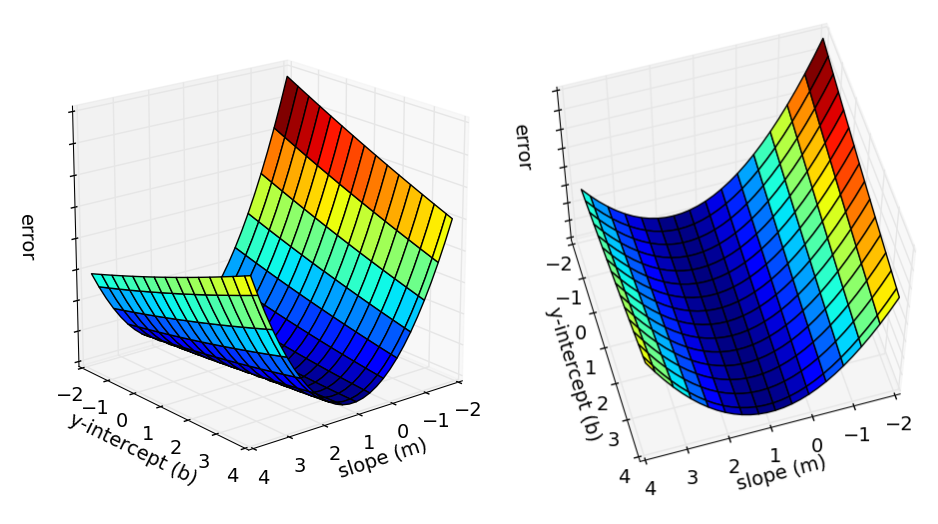
\includegraphics[width=0.5\textwidth]{figures/gradient_descent_error_surface.png}
  \caption{Error of paramater-pairs\cite{gradientdescent}}
  \label{fig:gradient_descent_error_surface}
\end{figure}

To find the minimum of our two-variable equation a good way is to use \textit{Gradient descent}\cite{wikigraddesc} algorithm. Gradient descent technique is an iterative algorithm used for find the local minimum of multi-variable functions. It is based on the observation, that if a multi-variable $F$ function is defined and differentiable in a neighborhood of a point $a$, F decreases fastest in the direction of the negative gradient of F($-\nabla F$). ($\nabla F$ is defined as: 
\begin{equation}
\nabla F= \dfrac{\partial F}{\partial x_1}\boldsymbol{e_1}+\dots+\dfrac{\partial F}{\partial x_n}\boldsymbol{e_n},
\end{equation} 
where $F:\mathbb{R}^{n}\to 	\mathbb{R}$ is n-dimensional function and $\boldsymbol{e_i}$,($i\in\{1\dots n\})$ are orthogonal unit vectors.

When gradient descent is applied for \textit{linear regression}, the first step to do is to calculate the partial derivatives of the $Error$ function for  $b$ and $m$ variables defining that.
\begin{align}
\dfrac{\partial Error}{\partial m} = \dfrac{2}{N}\sum_{i=1}^{N} -x_i(y_i-(mx_i+b)) \\
\dfrac{\partial Error}{\partial b} = \dfrac{2}{N}\sum_{i=1}^{N} -(y_i-(mx_i+b))
\end{align}
Using the partial derivative functions then we can initialize $b$ and $m$ variables, and let the gradient descent  algorithm march downhill on our error function towards the best line. In all iteration steps the algorithm modifies the values of the parameters according to partial derivatives, and results in a line with slightly lower error than the previous one. We also can define a rate specifying how big steps we take in the iteration steps. With smaller rate we progress slower, but with bigger rate we can miss the minimum. 
\cite{gradientdescent}%%(https://spin.atomicobject.com/2014/06/24/gradient-descent-linear-regression/)
\subsubsection{Iterative stream processing}
Typically data-parallel processing frameworks relies on  submitting a new job for each iteration, on adding new additional nodes to the already running acyclic dataflow graph, or adding feedback edges. 
\subsubsection{iterative fault tolerance}
Implementing fault tolerance in distributed data analysis systems is a complex problem. Optimal solutions\cite{allroadsleadtorome} among others depend on size of cluster, on hardware-characteristics, on duration of analyzing application or on duration of execution stages. The better solution will be different  as well if the failure happens in the first minute of the computation or if if the system crashes after a week of work.
Most solutions for fault tolerance introduce an overhead comparing to failure-free operation, as well as recovery procedures after a failure, all of these depends on parameters like the aforementioned ones.

Iterative recovery mechanism can be classified based according to their level of pessimism in three categories\cite{allroadsleadtorome}: \textit{Operator level pessimistic recovery},\textit{Iteration-level pessimistic recovery}, and \textit{optimistic recovery}, which is mostly applicable for ML-tasks. 

\paragraph{Operator-level recovery}, implemented for instance in MapReduce\cite{mapreduce}, backs-up the result of each individual stage of execution. Backing-up is done by write the whole result set either on local disk (at Map) or in distributed file system (Reduce). These writes incur a very high overhead for rapid recovery. For iterative tasks the amount of work in an iteration step is usually  much lower than in a typical MapReduce-job, therefore using this type of recovery is a real overkill.

\paragraph{Iteration level recovery} fits better to iterative tasks. Though the workload of an iteration is typically smaller than an ordinary MapReduce job, execution time across all iterations  may still be significant. Some graph-processing systems\cite{distgraphlab}\cite{pregel} therefore checkpoints the result of an iteration as whole. In case of failure all participating operator needs to revert to the last checkpointed state. By skipping checkpointing in a number of iterations, iteration-level recovery may provide the possibility to balance between higher overhead and better performance.

\paragraph{Optimistic recovery for Machine Learning}\cite{allroadsleadtorome} brings a different approach in fault tolerance by omit any kind of checkpointing. The idea is, that many Machine Learning algorithms does not need \textit{exactly once} semantics, thus if a number of tuples doesn't appear in the computation result the job will still converge.  This technique instead of reverting to a former state in case of failure applies a \textit{compensate} function on participating machines. The role of this function is to set the state of the entire application to a state from which the system can converge.

\paragraph{Naiad - timely dataflow : a simple but costly solution}
Microsoft's  distributed stream processing system, Naiad\cite{naiad} offers ability to perform iterative and incremental computations beyond providing high throughput and low latency.
The underlying concept of \textit{timely dataflows} implemented by Naiad system uses a new model of logical timestamps, which reflects structure in the graph topology such as loops, and makes the model suitable  for tracking progress in iterative algorithms. 

Before a tuple enters the pipelined computational system of timely dataflow, an external producer labels it with an integer \textit{epoch}, indicating a 
logical time window the record produced in. The producer can also notify operators (\textit{vertices} in Naiad) when from a given epoch no more message will be sent, and similarly the output vertices signals external consumers that processing an epoch is finished. In timely dataflow vertices are organized into possibly nested \textit{loop contexts}, and each cycle in the graph must be entirely contained by a loop context. Edges entering the loop context must pass through an \textit{ingress vertex}, edges leaving the loop has to pass through an \textit{egress vertex}, and a loop also has to contain at least one \textit{feedback vertex} which is not nested within any contained loop context.

Using constrains described  timely dataflow allowed designers of Naiad to define timestamps in the following way:
\begin{equation}
\tau=(\overbrace{e \in \mathbb{N}}^\text{epoch},\overbrace{\langle c_1,\dots,c_k \rangle \in \mathbb{N}^{k}}^\text{loop counters} ),
\end{equation} 
where each $c_i$ loop counter corresponds to one of the $k$ loop contexts, and explicitly distinguishing different iterations allows the system to forward progress as messages circulate around the dataflow graph. In this concept ingress, egress and feedback vertices act only on these timestamps as follows:
%%Systems using continuous operator model can use basically two different approach in checkpointing and backup. 
\begin{tabular}{l l l}
Vertex & Input timestamp & Output timestamp \\
\hline
Ingress & $(e,\langle c_1,\dots,c_k \rangle)$ & $(e,\langle c_1,\dots,c_k,0 \rangle)$\\
Egress & $(e,\langle c_1,\dots,c_k, c_{k+1} \rangle)$ & $(e,\langle c_1,\dots,c_k \rangle)$\\
Feedback & $(e,\langle c_1,\dots,c_k\rangle)$ & $(e,\langle c_1,\dots,c_k+1 \rangle)$\\
\end{tabular} 
Naiad uses a simple, stop-the-world approach in fault tolerance. Vertexes have to implement a checkpoint and a restore interface, and the system invokes these as appropriate to produce a consistent checkpoint across all workers. According to required durability of state backup, vertices can either log data as computation proceeds and thus execute checkpointing with lower latency, or make full checkpoints if required.

The system periodically requests vertices for checkpointing their state. Chackpointing of the computational system is done synchronously,  all vertices flushes their output buffers and do the computations on input than pauses work. After carrying out required level of checkpointing, the system resumes message delivery and computations. Checkpoint files can be saved to disk or replicated to other machines.

If a failure happens the system read latest checkpoint files and  all the vertices revert to last state saved in the checkpoint, and if it is necessary failed processes are being assigned to another node.

Designers of Naiad have chosen higher performance in the common case that there are no failures at the expense of availability in the event of failure. To bridge time gaps in processing caused by making checkpoints or failure recovery Naiad uses reliable message queue where it reads input from. 

\section{Iterative Fault-tolerance in Flink}
\subsection{Iterative dataflows in Flink}
Iterations and incremental processing are crucial for machine learning applications as well as for implementation of different graph processing algorithms. Iterations in Flink are implemented using \textit{iterative steps}, special operators that themselves can contain an execution graph. Flink makes difference on API level between two variant of iteration operator: simple textit{Iterate} and textit{Delta Iterate}.

The \textbf{iterate operator} implements a simple form of iterations, the step function consumes the entire result set of its upstream operator or the previous iteration then executes the iteration step and produces a the new partial solution. Step function is executed multiple times until a termination condition is met, that can be either a given maximum number of iterations or a \textit{convergence criteria}, which should be satisfied by a textit{custom aggregator}.
\begin{figure}[!ht]
  \centering    
      \includegraphics[width=0.5\textwidth]{figures/iterations_iterate_operator.png}
  \caption{Simple iterate operator in Flink\cite{flink_doc_iteration}}
  \label{fig:iterations_iterate_operator}
\end{figure}

\textbf{Delta iterate operator} covers the case of incremental computation. Incremental iterations selectively modify some elements of their solution set evolving the solution rather than fully recompute that. If this type of methods are applicable they lead to more efficient solutions, it splits the solution set into \textit{cold parts} and \textit{hot parts} and involve only hot parts into the next iteration steps. The majority of the solution set in many cases cools down quickly and thus fastens up the global execution significantly.
\begin{figure}[!ht]
  \centering    
      \includegraphics[width=0.5\textwidth]{figures/iterations_delta_iterate_operator.png}
  \caption{Delta iterate operator in Flink\cite{flink_doc_iteration}}
  \label{fig:iterations_iterate_operator}
\end{figure}
In parallel setups the step functions of multiple task instances are evaluated in parallel on different partitions of iteration state. One such parallel evaluation of on all the task instances forms a textit{superstep}, which is the granularity of synchronization, therefore all iteration task have need to be complete before initialization of the next superstep. Termination criteria is also evaluated at the barriers between supersteps.	
\cite{flink_doc_iteration}

\subsection{Asynchronous Barrier Snapshotting for cyclic dataflows}
Apache Flink uses Asynchronous Barrier Snapshotting what is based on the principle, that it is feasible to do snapshots without persisting channels' state, if we divide the execution into stages. 
It is possible to divide data streams into stages by injecting textit{barrier markers} a kind of control messages periodically, that are pushed throughout the whole execution graph to the sinks. Global snapshot of the systems are taken incrementally building on stages indicated by barrier markers. There are a couple of assumptions need to be met for ASB algorithms:
\begin{itemize}
\item Network channels need to be quasi-reliable, they have tor keep a FIFO delivery order, and can be blocked and unblocked. When a channel is blocked it has to be able to buffer all messages until it gets unblocked.
\item Tasks need to be enabled to order the channels to block, unblock and forward messages. They also has to be able to broadcast messages.
\end{itemize}
To execute a global snapshot a central coordinator injects the barrier to all the sources of execution graphs. When the source recieves the marker it takes  a snapshot of its current state, then forwards the barrier on all its downstreams.  When a non-source task receives a barrier on one of the input streams it blocks the stream and wait until the barrier is delivered on all the upstreams. When the task has received the barrier from all the upstream channel it executes the snapshot of its current state, broadcasts the barrier on all its downstream channels, and finally unblocks upstream channel and continues the computations.
\begin{figure}[!ht]
  \centering    
      \includegraphics[width=0.9\textwidth]{figures/abs_acyclic.png}
  \caption{Asynchronous Barrier Snapshotting in acyclic topology\cite{abs}}
  \label{fig:abs_acyclic}
\end{figure}
A snapshotting algorithms must guarantee \textit{termination} and \textit{feasibility}.(See subsection \ref{snapshotting})
\begin{description}
\item[Termination] is guaranteed by the DAG topology of acylic computation graph and reliability of the channels. Reliability ensures the if a barrier has been sent it will be eventually received as long as the receiver task is alive. The DAG topology furthermore guarantees that all tasks will receive the barrier on all the input channels.
\item[Feasibility] of the algorithms can be proved by showing, that a global snapshot contains only history of records that are processed up to the last stage. This is ensured by FIFO delivery and blocking of input channels ensuring that no post-shot record will be reflected in the state. 
\end{description}
\cite{abs}
In the presence of cycles in the execution graph ABS algorithm presented above will violate the requirement of \textit{termination}, since a task in a circle would wait indefinitely to receive the barriers on all of the input channels, resulting in deadlock. Moreover the records that are in transit within cycles would not be included in the snapshot contradicting the property of \textit{feasibility}. This second issue leads to the need to consistently include records in the circle in the snapshot to reach feasibility as well as restore them at recovery.
To address the problem of deadlocks we need to identify the set textit{back-edges} $L$  in the execution graph by static analysis. $L$ includes edges of the graph which has been already visited during \textit{depth-first search}. Without the $l_{bi} \in L$ back-edges $G(T, E\\L)$ execution graph is a DAG. that contains all tasks of in topology, on this part the former algorithm will work invariably. To deal with problem of records in transit there is a need to apply downstream backup logging the records received on back-edges during the snapshot, i.e. from the moment it forwards the barrier until it receives back on the back-edge.      
In the modified ABS algorithm  tasks with back-edge input creates a local copy of their state once they received the barrier from all their upstreams $(e \notin L)$ channels, then it broadcasts the barrier on all the downstreams, including the channels that are part of a circle. From that they log all records delivered from the back-edges until receives back the stage barrier too from them, incuding this way all pre-shot records in the current snapshot.  
\begin{figure}[!ht]
  \centering    
      \includegraphics[width=0.9\textwidth]{figures/abs_cyclic.png}
  \caption{Asynchronous Barrier Snapshotting in cyclic topology\cite{abs}}
  \label{fig:abs_cyclic}
\end{figure}
Again, to prove correctness of the algorithms we need to examine \textit{termination} and \textit{feasibility}:
\begin{description}

\item[Termination] of this modified is guaranteed. The problem of potential deadlocks is solved by forwarding barrier as soon as all the regular (non back-edge) channels delivered it. As the modified algorithm works as the unmodified one regarding the DAG partial graph (not considering additional logging), all tasks will eventually receive the barrier.
\item[Feasibility] may be proved in two steps. First local snapshots included in the global snapshot only contains state of task taken before any post-shot events received from regular upstreams. And second the downstream backup log included in the snapshot contains all records received on back-edges after the snapshot but before receiving back the barrier from back-edge.
\end{description} 
\cite{abs}
%%\subsection{Recovery}
%%TODO
%%\subsection{Exactly once}
%%TODO

\section{Performance}
In stream processing systems those essential aim is to answer queries with latency as low as possible a very important aspect is to measure the time overhead caused by  additional processes, that are necessary to carry out snapshotting. To evaluate this overhead I developed an implementation of linear regression using gradient descent
algorithm.
\subsection{Linear regression with Flink Streaming}
Linear regression is a method aiming to find a line best fitting to a given set of points. The implemented algorithm uses an iterative approach, where in each iteration step the result is a line a bit closer to the ideal one than in the previous iteration. To find a line with a smaller error in each step a well usable method is the gradient descent algorithm what I use to alter parameters until a given convergence criteria is met.(Algorithms in more detail in Section \ref{linearregression})
The set used to test the convergence of the algoritms consists of 21 points :
\begin{lstlisting}
 	P ={(0.5, 1.0 ),	( 1.0, 2.0 ),
		( 2.0, 4.0 ),	( 3.0, 6.0 ),
		( 4.0, 8.0 ),	(5.0, 10.0 ),
		( 6.0, 12.0 ),	( 7.0, 14.0 ),
		( 8.0, 16.0 ),	(9.0, 18.0 ),
		( 10.0, 20.0 ),	( -0.08, -0.16 ),
		( 0.13, 0.26 ),	( -1.17, -2.35 ),
		( 1.72, 3.45 ),	( 1.70, 3.41 ),
		( 1.20, 2.41 ),	( -0.59, -1.18 ),
		( 0.28, 0.57 ),	( 1.65, 3.30 ),
		( -0.55, -1.08 )}
\end{lstlisting}
The target line equation is $y=2x+0$.

The algorithm first read the iterates over the same point set until convergence. 
\begin{lstlisting}
 val iteration = data.iterate { data =>
      
      // compute a single step using every sample
      val updated = data.flatMap(new SubUpdate) /
        .timeWindowAll(Time.seconds(1))
        // sum up all the steps in window
        .reduce(new UpdateAccumulator) 
        // average the steps and update all parameters
        .map(new Update)
        .broadcast

      val connected = data.connect(updated)
        .map(x => x, x => Right(x))
        .split(new IterationSelector)
      (connected.select("iterate"), connected.select("output"))
    }
\end{lstlisting}
As a data entered in the computational pipeline the algorithm maps each point to a displacement to apply on parameters of the line. The displacement is defined by the $SubUbdate$ function, which computes the gradient of the point:
\begin{lstlisting}
val delta_0 = - 0.1 * (data.y - (parameter.theta0 
		+ (parameter.theta1 * data.x)) )
val delta_1 = - 0.1 * data.x * (data.y- ( (parameter.theta1 * data.x) 
		+ parameter.theta0 ) )
val new_parameter = new Params(delta_0, delta_1)
\end{lstlisting}
The displacement vectors issued by $SubUpdate$ are collected together and summerized in every seconds, than the sum is applied to parameters of the line. The new line than must be broadcasted between all nodes.

At the end of the iteration step the Flink API enable the algorithm to select the \textit{cooled down parts} and continue the computation only on \textit{hot parts} of the input set, but in this case we need all the data to met the convergence criteria, and we send back all the records in $IterationSelector$.    


 
      